%中間審査概要テンプレート ver. 3.0

\documentclass[uplatex,twocolumn,dvipdfmx]{jsarticle}
\usepackage[top=22mm,bottom=22mm,left=22mm,right=22mm]{geometry}
\setlength{\columnsep}{10mm}
\usepackage[T1]{fontenc}
\usepackage{txfonts}
\usepackage[expert,deluxe]{otf}
\usepackage[dvipdfmx,hiresbb]{graphicx}
\usepackage[dvipdfmx]{hyperref}
\usepackage{pxjahyper}
\usepackage{secdot}





%タイトルと学生番号,名前だけ編集すること
\title{\vspace{-5mm}\fontsize{14pt}{0pt}\selectfont  ゲーム攻略Wikiにおけるプロジェクトマネジメント状況の分析}
\author{\normalsize プロジェクトマネジメントコース 矢吹研究室 1342014 泉 雄太}
\date{}
\pagestyle{empty}
\begin{document}
\fontsize{10.5pt}{\baselineskip}\selectfont
\maketitle





%以下が本文
\section{序論}

wikiを使用しているサイトは通常,特定あるいは不特定多数の人間が集まって作られている.そのためこれらを作成する過程ではプロジェクトマネジメントが行われているのではないかと考え,本研究ではゲーム攻略wikiを対象にした調査を行う.

なお,ゲーム攻略wikiには期限がないため,厳密にいえばプロジェクトの定義から外れている.しかし,人が集まって一つのモノを作るという性質上,マネジメントが行われているのではないかと仮定して研究を行う.


\section{目的}

データマイニングにより,ゲーム攻略wikiにおけるプロジェクトマネジメントの状況を分析し,ネット上での不特定多数によるプロジェクトの新たな特性の発見する.

\section{手法}

ゲーム攻略wiki内の編集履歴から,クローラーを用いて編集者ID,編集回数,編集文字数を取得する.次に,Rを用いて前述のデータからヒストグラムを作成する.作成したヒストグラムは,別の研究で作成されたWikipediaのヒストグラムと比較する.

\section{結果}

%図の挿入
\begin{figure}[thbp]
\begin{tabular}{cc}
 \begin{minipage}{0.5\hsize}
  \begin{center}
   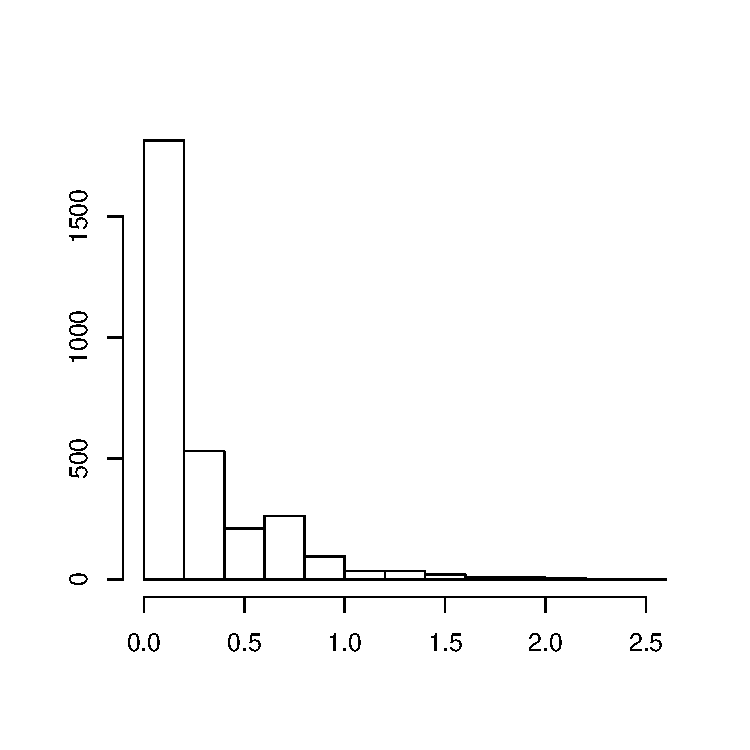
\includegraphics[width=45mm]{logk.pdf}
   \caption{編集回数のヒストグラム}
   \label{K}
  \end{center}
 \end{minipage}%
 \begin{minipage}{0.5\hsize}
  \begin{center}
   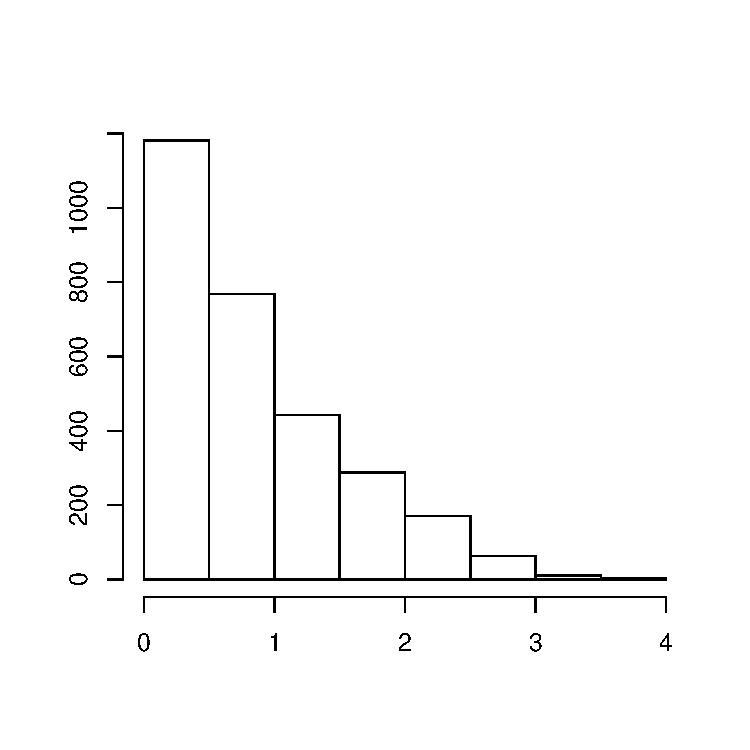
\includegraphics[width=45mm]{logm.pdf}
   \caption{1人ごとの編集文字数のヒストグラム}
   \label{M}
  \end{center}
 \end{minipage}
 \end{tabular}
 \end{figure}

「The Elder Scrolls V Skyrim」\cite{wikipedia}の日本語版攻略wiki\cite{wiki}を対象に調査をおこなった.同wikiから得たデータをもとに「1人の編集者が何回の編集をおこなったかについてのヒストグラム.(図\ref{K})」と「1人の編集者が何文字編集したかについてのヒストグラム.(図\ref{M})」を作成した.なお,データの幅が大きかったため,ヒストグラムはすべて対数化した.

wikipediaとの比較は,編集者ごとの編集回数のヒストグラムで行った.(手に入ったのがそのデータだけのため.)

\section{考察}

1人当たりの編集文字数と編集回数をみると,多数の貢献度が低い編集者と,ごく少数の貢献度が高い編集者で構成されていると読み取れる.これは不特定多数でのオープンな作業の特徴であるといえ,クローズドな作業で適用されやすい2:8:2の法則が当てはまっていないことがわかる.

wikipediaとの比較では,ゲーム攻略wikiとの違いは見受けられないことがわかる.しかし,現時点では比較できる情報が編集者ごとの編集回数のみであるため,情報が不足しているといえる.

\section{結論}

本研究では不特定多数かつオープンなプロジェクトが,独特な組織体系をもつことがわかった.しかし,解析できていないデータ領域も多数ある.今後はそういったデータの解析を進め,不特定多数かつオープンなプロジェクトの新たな特性や,ゲームwiki特有の特性が見つかることが期待される.

\bibliographystyle{junsrt}
\bibliography{biblio}%「biblio.bib」というファイルが必要.

\end{document}
